\documentclass[a4paper]{article}

%% Language and font encodings
\usepackage[spanish]{babel}
\usepackage[utf8x]{inputenc}
\usepackage[T1]{fontenc}

%% Sets page size and margins
\usepackage[a4paper,top=3cm,bottom=2cm,left=3cm,right=3cm,marginparwidth=2cm]{geometry}

%% Useful packages
\usepackage{amsmath}
\usepackage{graphicx}
\usepackage[colorinlistoftodos]{todonotes}
\usepackage[colorlinks=true, allcolors=blue]{hyperref}
\usepackage{array}
\usepackage{float}



\title{COMPARATIVA DE TÉCNICAS DE PROCESAMIENTO DE IMÁGENES PARA LA DETECCIÓN DE PEATONES CON SVM}
\author{Álvaro Ruiz Gutiérrez, Lidia Jiménez Soriano, Víctor Flores González, Óscar Menéndez Márquez}

\begin{document}
\maketitle

\begin{abstract}
  \noindent En este trabajo se analiza y compara la eficiencia de cuatro métodos de extracción de características en imágenes: Harris Corner Detection, SURF, SIFT y HOG, aplicados a la detección de peatones mediante un modelo SVM preentrenado. 
  Se estudia la teoría detrás de cada método, extrayendo y explicando sus principios fundamentales de manera didáctica. Posteriormente, se implementan o adaptan implementaciones existentes, 
  detallando los parámetros utilizados y los efectos que tienen en el rendimiento del modelo. Para evaluar la eficiencia de cada método, se definen métricas clave como la precisión y tiempo de procesamiento. 
  Se presentan los resultados obtenidos mediante experimentación con un conjunto de datos de imágenes, analizando el impacto de cada técnica en la identificación de peatones. Finalmente, se expone de manera clara la 
  comparativa de los métodos estudiados, destacando sus ventajas y desventajas en función de los resultados obtenidos.  
 
 \hspace{1cm}
 
 \noindent \textbf{Palabras clave:} 
 Harris Corner Detection,SURF , SIFT, HOG, procesamiento de imágenes, detección de peatones, SVM.
 \end{abstract}
 


 \section{Introducción}

 El procesamiento de imágenes digitales es un campo clave dentro de la visión por computador, con aplicaciones en reconocimiento de patrones, inteligencia artificial y análisis de imágenes. Dentro de este ámbito, la detección de objetos y, en particular, la identificación de peatones, representa un desafío fundamental con implicaciones en seguridad, movilidad y automatización. 
 \par \hspace{1cm}

 Este trabajo se centra en el estudio y comparación de cuatro técnicas de extracción de características utilizadas en la identificación de peatones: \textbf{Harris Corner Detection}, \textbf{SURF (Speeded Up Robust Features)}, \textbf{SIFT (Scale-Invariant Feature Transform)} y \textbf{HOG (Histogram of Oriented Gradients)}. Estas técnicas permiten identificar estructuras relevantes en una imagen, facilitando su uso en tareas de reconocimiento y clasificación. Para evaluar su rendimiento, se utilizará un \textbf{modelo SVM (Support Vector Machine) preentrenado}, el cual procesará los descriptores generados por cada método para realizar la identificación de peatones en imágenes. 
 \par \hspace{1cm}


 El \textbf{objetivo} principal de este trabajo es ofrecer una explicación didáctica de los métodos estudiados, tanto desde un punto de vista teórico como práctico. Para ello, el desarrollo del proyecto se estructura en tres fases clave:
 
 \begin{itemize}
     \item \textbf{Análisis teórico:} Se investigarán los principios fundamentales de cada método, extrayendo las ideas principales de fuentes científicas.
     \item \textbf{Implementación práctica:} Se desarrollará o adaptará la implementación existente de cada técnica, detallando los pasos intermedios, el significado de los parámetros y la experimentación con distintas configuraciones.
     \item \textbf{Presentación didáctica:} Se explicarán de forma estructurada todos los pasos necesarios para la detección de peatones utilizando cada método, complementando con ejemplos gráficos y análisis de resultados.
 \end{itemize}
 
 Dado que el desarrollo del trabajo está orientado a la investigación y aplicación de técnicas avanzadas no vistas en clase, se apoyará en artículos científicos recientes. La \textbf{planificación} y ejecución del proyecto se realizará en un equipo de trabajo compuesto por 4 alumnos
 ,distribuyendo \textbf{70 horas por persona}. Además, se utilizarán herramientas de gestión de proyectos para organizar y documentar las tareas realizadas, asegurando un seguimiento adecuado de los 
 avances. Concretamente, se utilizará GitHub como repositorio del código fuente y documentación, Clockify para el registro y seguimiento de horas y tareas, y Microsoft Project para realizar una planificación previa precisa de las fases, hitos y actividades previstas.
 \newpage

 \section{Planteamiento teórico}
 \par\vspace{0.5cm}

 El problema abordado se centra en la detección automatizada de peatones a partir de imágenes digitales mediante técnicas de procesamiento de imágenes como \textbf{Harris}, \textbf{SURF}, \textbf{SIFT} y \textbf{HOG}. Esta tarea es fundamental en múltiples aplicaciones, 
 como la seguridad vial, la monitorización del tráfico y la visión por computadora en sistemas autónomos. La detección 
 precisa y eficiente de peatones permite mejorar la toma de decisiones en entornos urbanos, reducir accidentes o incluso optimizar sistemas de asistencia a la conducción. 
 \par\vspace{0.5cm}

 Para abordar este problema, se han implementado y evaluado los algoritmos mencionados, 
 los cuales permiten extraer características distintivas de las imágenes con el objetivo de identificar patrones asociados 
 a la presencia de peatones. En esta sección, se describirá en profundidad el funcionamiento de cada uno de estos algoritmos, analizando sus fundamentos teóricos, principios matemáticos y ventajas frente a otros enfoques. Esta base teórica servirá como punto de partida para su posterior implementación y evaluación experimental.
 

  \subsection{Harris Corner Detection}
  \par\vspace{0.5cm}

  El algoritmo \textbf{HARRIS} (Harris Corner Detection) es un método ampliamente utilizado en visión por computadora para la detección de esquinas y puntos de interés en imágenes. Fue desarrollado por \textit{Chris Harris} y \textit{Mike Stephens} en 1988 
  y se basa en la idea de que las esquinas son puntos donde la intensidad de la imagen cambia significativamente en múltiples direcciones. Este algoritmo es especialmente útil para tareas como el seguimiento de objetos, la reconstrucción 3D y la detección 
  de características invariantes a escala y rotación.

  \par\vspace{0.5cm}
  \textbf{Fundamentos matemáticos}
  \par\vspace{0.5cm}
  
  El algoritmo Harris se basa en varios principios matemáticos que son los pilares de su funcionamiento.
   A continuación, se presentan algunos de los conceptos clave:
  
  \begin{itemize}
      \item \textbf{Extracción de los autovectores y autovalores:}  
      El algoritmo Harris utiliza la matriz de autocorrelación para identificar esquinas en la imagen. El porque 
      de utilizar la matriz de autocorrelación es que, al calcular los autovectores y autovalores de esta matriz, se pueden identificar puntos donde la intensidad de la imagen cambia significativamente en múltiples direcciones.
      La imagen que se muestra a continuación ilustra como varia los autovalores y autovectores en función de la intensidad de la imagen.
      \begin{figure}[H]
        \centering
        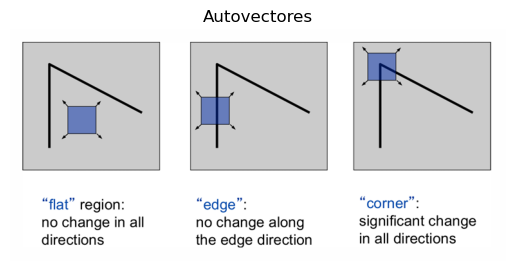
\includegraphics[width=1.1\textwidth]{images/harris_autovectores.png}
        \caption{Proceso de la piramide de diferencia gaussiana.}
        
    \end{figure}
      
    \item Para el cálculo de dichos autovectores y autovalores, se utiliza la matriz de autocorrelación \(M\) que se define como:
    \[
        M \cdot x = \lambda \cdot x
    \]
    
    Donde:
    \begin{itemize}
        \item \(M\) es la matriz de autocorrelación de la imagen.
        \item \(x\) es nuestra matriz de autovectores.
        \item \(\lambda\) es el llamado autovalor, es decir, cuánto aumenta en cada dirección el autovector.
    \end{itemize}

    Los autovectores y autovalores se obtienen resolviendo la siguiente igualdad.
    
        \[
        \det(M - \lambda I) = 0
        \]

        \[
        \det(M - \lambda I) = \det\left(
        \begin{bmatrix}
        a_{11} - \lambda & a_{12} \\
        a_{21} & a_{22} - \lambda
        \end{bmatrix}
        \right) = 0
        \]

        Los elementos \(a_n\) son los elementos de la matriz de autocorrelación \(M\) y \(\lambda\) es el autovalor. 
        \(lambda_max\) corresponde al autovalor máximo y \(lambda_min\) al autovalor mínimo, es decir, cuanto aumenta la intensidad de la imagen en cada dirección.

        \[
        (a_{11} - \lambda)(a_{22} - \lambda) - a_{12} a_{21} = 0
        \]

        Como se trata de un polinomio de segundo grado, podemos obtener fácilmente las soluciones:

        \[
        \lambda_{\text{max}} = \frac{1}{2} \left(a_{11} + a_{22} + \sqrt{4a_{12}a_{21} + (a_{11} - a_{22})^2}\right)
        \]

        \[
        \lambda_{\text{min}} = \frac{1}{2} \left(a_{11} + a_{22} - \sqrt{4a_{12}a_{21} + (a_{11} - a_{22})^2}\right)
        \]


      \item \textbf{Calculo del gradiente de la imagen:}  
        Debemos calcular el gradiente de la imagen para poder calcular la matriz de autocorrelación. Para cada pixel
        de la imagen, dicho gradiente se calcula como:
      
        \[
        \nabla f(x, y) =
        \begin{bmatrix}
        \frac{\partial f(x, y)}{\partial x} \\
        \frac{\partial f(x, y)}{\partial y}
        \end{bmatrix}
        \]

        Dado que este cálculo también es relativamente complejo y costoso, podemos aproximarlo de la siguiente manera:

        \[
        \text{Filtro de Sobel} \approx \nabla f(x, y) =
        \begin{bmatrix}
        \frac{\partial f(x, y)}{\partial x} \\
        \frac{\partial f(x, y)}{\partial y}
        \end{bmatrix}
        \approx
        \begin{bmatrix}
        I_x \\
        I_y
        \end{bmatrix}
        \]

        \textbf{Nota:} El resultado es en realidad una matriz con \(f_x\) y \(f_y\), pero se ha representado como \(I_x\) e \(I_y\) por simplicidad.

      
      \item \textbf{Calculo de la matriz de autocorrelación:}  
      
      Debemos realizar el siguiente para obtener la matriz de autocorrelación \(M\) para cada pixel de la imagen:

            \[
        A = \sum_{x, y} w(x, y)
        \begin{bmatrix}
        I_x^2 & I_x I_y \\
        I_x I_y & I_y^2
        \end{bmatrix}
        \]

        Para simplificar, evitamos el uso explícito de la función ventana \(w(x, y)\), y aprovechamos que ya contamos con los valores de \(I_x\) e \(I_y\), por lo que simplemente calculamos sus productos.

        \item \textbf{Calculo de las notas Harris para cada pixel:} 
    
        Finalmente, para cada pixel de la imagen, calculamos la nota Harris \(R\) Esta nota representa
        el valor de "esquinidad" de cada pixel, es decir, que tan "esquina" es el pixel, a mayor valor, mayor esquinidad.

        \[
        f(x, y) = \lambda_{\text{min}} \lambda_{\text{max}} - \kappa (\lambda_{\text{min}} + \lambda_{\text{max}})^2
        \]

        \textbf{Nota:} El valor \(\kappa\) corresponde al parámetro \(k\) de la ecuación original de Harris, que se utiliza para ajustar la sensibilidad del detector. Un valor comúnmente utilizado es \(k = 0.04\).

        Afortunadamente, el valor de Harris se puede calcular de una manera equivalente pero más sencilla:

        \[
        f(x, y) = \det(A) - \kappa \, \text{tr}(A)^2 = a_{11} a_{22} - a_{12} a_{21} - \kappa (a_{11} + a_{22})^2
        \]

    Esta formulación es mucho más simple y se puede obtener fácilmente mediante el uso de filtros de gradiente como el filtro de Sobel.

  \end{itemize}

  \par\vspace{0.5cm}
  \textbf{Ventajas de HARRIS}
  \par\vspace{0.5cm}
  
  El algoritmo HARRIS presenta varias ventajas en comparación con otros métodos de detección de características:
  
  \begin{itemize}
      \item \textbf{Robustez frente al ruido:}  
      Gracias al uso de filtros de suavizado y la matriz de autocorrelación, el algoritmo es menos sensible al ruido en la imagen, lo que permite una detección más precisa de esquinas.
      
      \item \textbf{Alta precisión en la detección de esquinas:}  
      Identifica puntos donde las variaciones de intensidad son altas en múltiples direcciones, lo que corresponde a esquinas reales con muy buena exactitud.
      
      \item \textbf{Invariancia a la rotación:}  
      El detector es invariante a rotaciones: si rotas la imagen, las esquinas detectadas rotarán de manera consistente. Esto es útil para tareas como emparejamiento de imágenes o reconstrucción 3D.
      
      \item \textbf{Bajo costo computacional:}  
      El dectector usa calculos de gradientes simples mediante filtros de Sobel, además de calculos sencillos como las notas Harris, lo que lo hace eficiente en términos de tiempo de procesamiento.
      
      \item \textbf{Respuesta continua:}
      La salida del detector es continua, es decir, no se limite a un conjunto binario de pixeles, si no que ofrece una matriz
      de valores que representan la "esquinidad" de cada pixel. Esto permite ajustar el umbral de detección según las necesidades del problema, además de ofrecer ordenación de los puntos detectados.  
    \end{itemize}
  
  \par\vspace{0.5cm}


  \subsection{SURF (Speeded-Up Robust Features)}
  \par\vspace{0.5cm}

  \subsection{SIFT (Scale-Invariant Feature Transform)}
  \par\vspace{0.5cm}
  
  El algoritmo \textbf{SIFT} (Scale-Invariant Feature Transform) es una técnica ampliamente utilizada en visión por computadora para la detección y descripción de características en imágenes. Fue desarrollado por \textit{David Lowe} en 1999 y destaca por su capacidad de identificar puntos clave en una imagen de manera robusta frente a transformaciones como cambios de escala, rotación e iluminación. Gracias a estas propiedades, SIFT se ha convertido en una herramienta fundamental para aplicaciones como el reconocimiento de objetos, la detección de patrones y el emparejamiento de imágenes.
  
  \par\vspace{0.5cm}
  \textbf{Fundamentos teóricos}
  \par\vspace{0.5cm}
  
  El algoritmo SIFT se basa en la extracción de puntos característicos (keypoints) de una imagen y la generación de descriptores asociados a ellos. Este proceso se realiza en varias etapas, las cuales garantizan la invariancia a escala y a rotación.
  
  \begin{itemize}
      \item \textbf{Construcción de la Pirámide Gaussiana:}  
      Se aplican sucesivas convoluciones con un filtro gaussiano para generar versiones suavizadas de la imagen en diferentes escalas. Este proceso permite analizar la imagen a distintos niveles de detalle, lo que hace que los puntos característicos sean robustos a cambios de tamaño y desenfoque.
      
      \item \textbf{Construcción de la Pirámide de Diferencia de Gaussianos (DoG):}  
      Se calculan diferencias entre imágenes suavizadas consecutivas de la pirámide gaussiana. Esta operación permite resaltar bordes y estructuras significativas en la imagen, facilitando la detección de puntos clave.
      
      \begin{figure}[H]
        \centering
        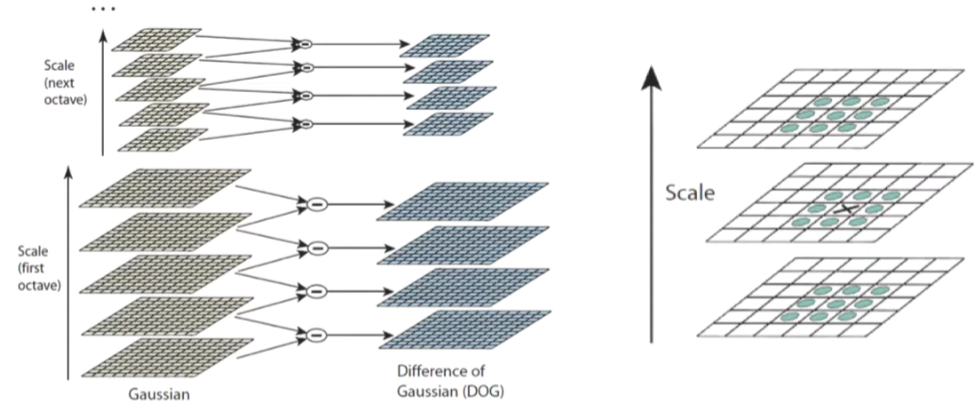
\includegraphics[width=1.1\textwidth]{images/sift_gauss.png}
        \caption{Proceso de la piramide de diferencia gaussiana.}
    \end{figure}
    
      \item \textbf{Detección de keypoints:}  
      Se identifican los puntos extremos en la pirámide DoG, comparando cada píxel con sus vecinos en los niveles superior e inferior de la pirámide, así como en su entorno local. Los puntos seleccionados se someten a un proceso de refinamiento para descartar aquellos con bajo contraste o situados en bordes poco definidos.
      
      \item \textbf{Asignación de orientación:}  
      A cada keypoint se le asigna una orientación dominante basada en la distribución de gradientes en su vecindad. Para ello, se calcula el gradiente horizontal y vertical, y se calcula el histograma de orientaciones del gradiente en una ventana centrada en el punto en la escala en la que se ha detectado. La orientación 
      se discretiza en 36 intervalos y se van acumulando las amplitudes del gradiente en cada ángulo detectado. Esto permite que el algoritmo sea invariante a rotaciones.
      \begin{figure}[H]
        \centering
        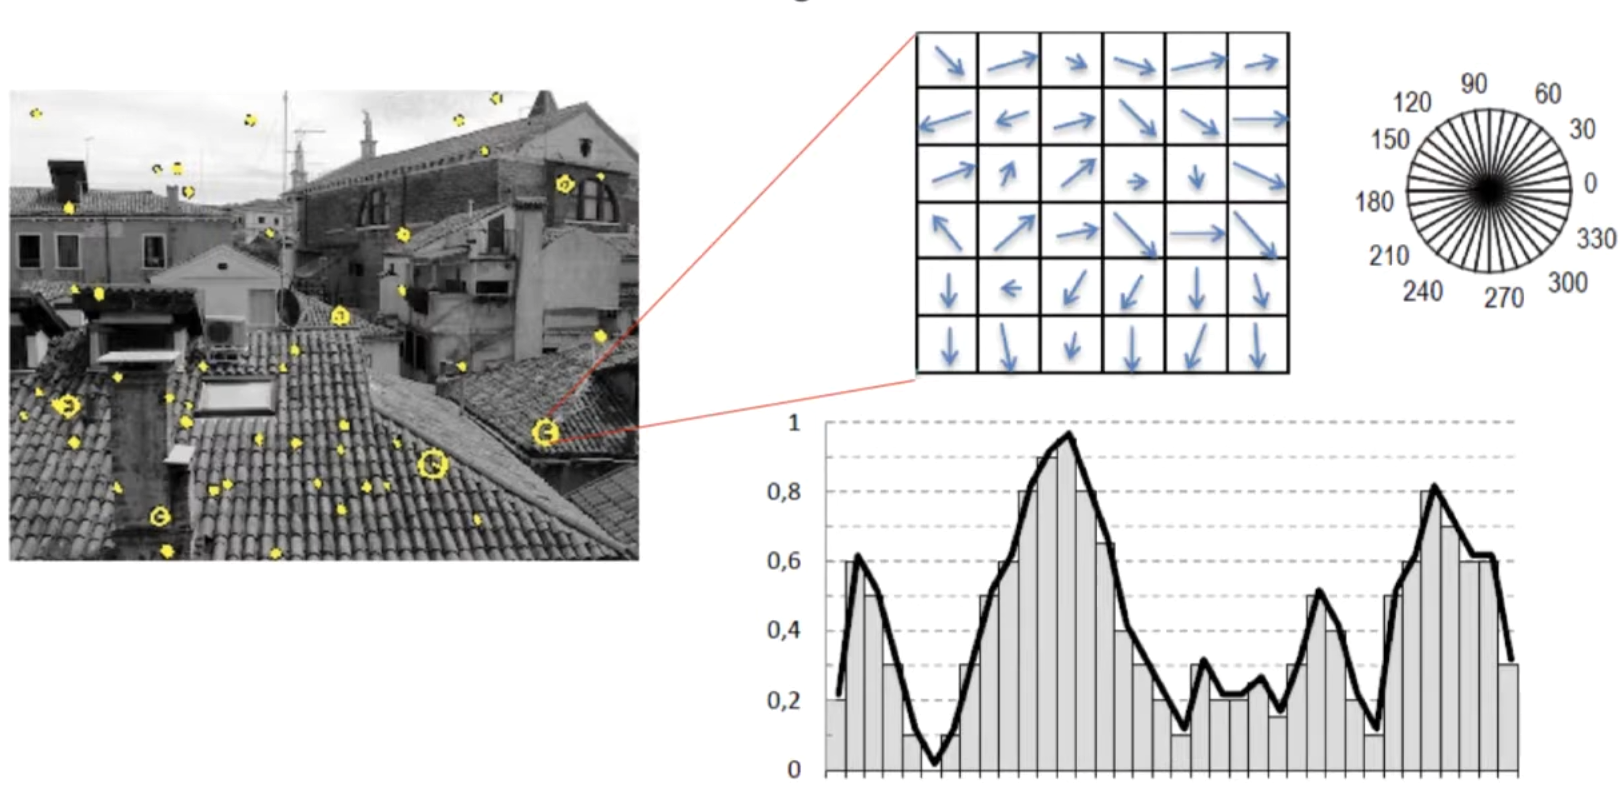
\includegraphics[width=1.1\textwidth]{images/sift_orientacion.png}
        \caption{Proceso de orientación de un keypoint.}
    \end{figure}


    \item \textbf{Generación del descriptor SIFT:}  
    Para representar de manera robusta un keypoint, se genera un descriptor basado en la distribución de los gradientes dentro de una ventana centrada en dicho punto.  
    Esta región se divide en una cuadrícula de \(4 \times 4\) celdas, formando un total de 16 subregiones.  
    En cada subregión se calcula un histograma de orientaciones de gradientes con 8 direcciones posibles.  
    Finalmente, los 16 histogramas se concatenan en un único vector de características de 128 dimensiones, dado que proviene de la combinación de las 16 subregiones (\(4 \times 4\)) y las 8 direcciones (\(16 \times 8 = 128\)).  
    Este descriptor permite identificar y comparar keypoints de manera robusta frente a variaciones en escala, rotación e iluminación.

   
      \begin{figure}[H]
        \centering
        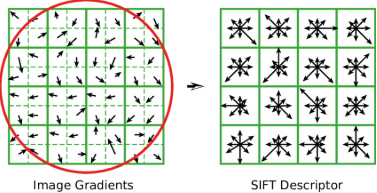
\includegraphics[width=0.7\textwidth]{images/sift_descrip.png}
        \caption{Keypoint Descriptor.}
    \end{figure}

    \end{itemize}
  
  \par\vspace{0.5cm}
  \textbf{Fundamentos matemáticos}
  \par\vspace{0.5cm}
  
  El algoritmo SIFT se basa en varios principios matemáticos que garantizan su eficacia en la detección y descripción de características. A continuación, se presentan algunos de los conceptos clave:
  
  \begin{itemize}
      \item \textbf{Filtro Gaussiano:}  
      La función gaussiana en dos dimensiones está definida por:
      \[
      G(x, y, \sigma) = \frac{1}{2\pi\sigma^2} \exp\left(-\frac{x^2 + y^2}{2\sigma^2}\right)
      \]
      donde \(\sigma\) controla el nivel de suavizado aplicado a la imagen.
      
      \item \textbf{Diferencia de Gaussianos (DoG):}  
      Se define como la resta entre dos imágenes suavizadas con diferentes valores de \(\sigma\):
      \[
      DoG(x, y, \sigma) = G(x, y, \sigma_2) - G(x, y, \sigma_1)
      \]
      Esta operación resalta los cambios de intensidad y permite la detección de keypoints.
      
      \item \textbf{Cálculo del gradiente:}  
      Para determinar la orientación de un keypoint, se calcula el gradiente de la imagen en cada píxel utilizando:
      \[
      m(x, y) = \sqrt{(L(x+1, y) - L(x-1, y))^2 + (L(x, y+1) - L(x, y-1))^2}
      \]
      \[
      \theta(x, y) = \tan^{-1} \left(\frac{L(x, y+1) - L(x, y-1)}{L(x+1, y) - L(x-1, y)}\right)
      \]
      donde \(m(x, y)\) representa la magnitud del gradiente y \(\theta(x, y)\) su dirección.
      
      \item \textbf{Generación del descriptor SIFT:}  
      El descriptor de cada keypoint como se explicó anteriormente, se forma a partir de histogramas de gradientes calculados en una ventana de \(16\times16\) píxeles alrededor del punto de interés. La ventana se subdivide en \(4\times4\) celdas y en cada celda se calcula un histograma de 8 orientaciones, generando un vector de:
      \[
      4 \times 4 \times 8 = 128
      \]
      dimensiones, que representa la información local de la imagen.
  \end{itemize}
  
  \par\vspace{0.5cm}
  \textbf{Ventajas de SIFT}
  \par\vspace{0.5cm}
  
  El algoritmo SIFT presenta varias ventajas en comparación con otros métodos de detección de características:
  
  \begin{itemize}
      \item \textbf{Invariancia a escala y rotación:}  
      Gracias a la construcción de la pirámide gaussiana y la asignación de orientación, los keypoints detectados son robustos a cambios de tamaño y rotación en la imagen.
      
      \item \textbf{Alta discriminación y robustez:}  
      Los descriptores SIFT tienen una alta capacidad para diferenciar objetos en diferentes condiciones de iluminación y perspectiva.
      
      \item \textbf{Resistencia a ruido y oclusiones parciales:}  
      Debido a su método de detección basado en diferencias de gaussianos y análisis de gradientes, SIFT es menos sensible al ruido y sigue funcionando incluso cuando partes de la imagen están ocultas.
      
      \item \textbf{Aplicabilidad en reconocimiento de patrones y emparejamiento de imágenes:}  
      El uso de descriptores de 128 dimensiones permite realizar comparaciones eficientes entre imágenes, facilitando tareas como el reconocimiento de objetos.
  \end{itemize}
  
  \par\vspace{0.5cm}
 


  \subsection{HOG (Histogram of Oriented Gradients)}
  \par\vspace{0.5cm}

  El descriptor \textbf{HOG}, propuesto por \textit{Dalal y Triggs} en 2005, es una técnica ampliamente utilizada para la detección de humanos en imágenes. Su éxito se basa en la idea de que la apariencia y la forma de los objetos, y en particular de las personas, pueden caracterizarse de manera efectiva mediante la distribución de gradientes o bordes. Esta representación es robusta frente a cambios en la iluminación y pequeñas variaciones en la geometría de la imagen, lo que la convierte en una herramienta idónea para alimentar clasificadores como el SVM

  \par\vspace{0.5cm}
  \textbf{Fundamentos teóricos y matemáticos}
  \par\vspace{0.5cm}

  El algoritmo HOG se fundamenta en los siguientes conceptos:

  \begin{itemize}
    \item \textbf{Cálculo de Gradientes:} 
    La primera etapa del proceso consiste en convertir la imagen a escala de grises y calcular, para cada píxel, la magnitud y la orientación del gradiente. Utilizando operadores como el de Sobel, se obtienen dos imágenes: una con las derivadas en la dirección horizontal (Gx) y otra en la vertical (Gy). A partir de estas, se calcula la magnitud M y la orientación \(\theta\) según:
    \[
    M(x,y) = \sqrt{G_x(x,y)^2 + G_y(x,y)^2}
    \]
    \[
    \theta(x,y) = \arctan\left(\frac{G_y(x,y)}{G_x(x,y)}\right) \times \frac{180}{\pi}
    \]
    Los ángulos se ajustan al rango \textbf{[0,180°)} para mantener la invarianza ante la dirección (ya que un borde tiene la misma apariencia tanto en una dirección como en la opuesta).
    \item \textbf{División en Celdas:}
    La imagen se divide en pequeñas regiones (celdas), típicamente de \(8\times8\) o \(16\times16\) píxeles, en las que se construye un histograma de orientaciones. Cada celda produce un histograma donde se acumulan las magnitudes de los gradientes de los píxeles, distribuidas en un número fijo de intervalos (por ejemplo, 9 bins, donde cada bin abarca 20°).
    \item \textbf{Normalización de Bloques:}
    Para reducir los efectos de variaciones en iluminación y contraste, se agrupan las celdas en bloques solapados (por ejemplo, \(2\times2\) celdas). Cada bloque se aplana en un vector y se normaliza (usualmente mediante la normalización L2 o L2-Hys) según:
    \[
    v_{\text{norm}} = \frac{v}{\|v\|_2 + \epsilon}
    \]
    donde \textbf{v} es el vector formado por la concatenación de los histogramas de las celdas del bloque y \textbf{\(\epsilon\)} es una pequeña constante para evitar la división por cero. La normalización asegura que el descriptor sea menos sensible a cambios en la iluminación.
    \item \textbf{Concatenación del Descriptor HOG:}
    Los vectores normalizados de todos los bloques se concatenan para formar el descriptor HOG final, que representa de forma global la distribución de gradientes en la imagen. Este descriptor es utilizado para alimentar el clasificador (SVM) que se encarga de diferenciar entre imágenes con y sin peatones.
\end{itemize}

\par\vspace{0.5cm}
\textbf{Ventajas de HOG}
\par\vspace{0.5cm}

El descriptor HOG presenta varias ventajas en comparación con otros métodos de detección de características:

\begin{itemize}
    \item \textbf{Robustez a Variaciones de Iluminación:}
    La normalización de bloques reduce el impacto de cambios en el brillo y contraste.
    \item \textbf{Invarianza a Pequeñas Variaciones Geométricas:}
    La estructura local capturada por las celdas y bloques permite que el descriptor sea relativamente invariante a pequeñas transformaciones, desplazamientos o deformaciones.
    \item \textbf{Simplicidad y Eficiencia:}
    HOG es relativamente sencillo de implementar y, a pesar de requerir cálculos intensivos de gradientes, puede optimizarse para aplicaciones en tiempo real. 
\end{itemize}

\par\vspace{0.5cm}


\newpage

\section{Implementación}

\subsection{Tecnologías}

Para este proyecto se ha utilizado Python como lenguaje de programación junto con varias librerías especializadas en procesamiento de imágenes, aprendizaje automático y visualización de datos. A continuación, se detallan las principales tecnologías empleadas:

\begin{itemize}
\item \textbf{OpenCV} \href{https://opencv.org/}{(web oficial)}: Biblioteca de código abierto para visión por computadora y procesamiento de imágenes. Se utilizó para la lectura, preprocesamiento y transformaciones de las imágenes.
\item \textbf{Numpy} \href{https://numpy.org/}{(web oficial)}: Biblioteca especializada en cálculo numérico y gestión de matrices multidimensionales. Se usó para la manipulación de datos y cálculos matemáticos en la transformación de imágenes.
\item \textbf{Matplotlib} \href{https://matplotlib.org/}{(web oficial)}: Biblioteca de visualización de datos. Se empleó principalmente para representar imágenes, mostrar los puntos de interés detectados y visualizar los resultados obtenidos.
\item \textbf{Scikit-image} \href{https://scikit-image.org/}{(web oficial)}: Biblioteca de procesamiento de imágenes que proporciona herramientas adicionales para realizar operaciones de filtrado, detección de bordes y transformaciones de imágenes.
\item \textbf{Scikit-learn} \href{https://scikit-learn.org/}{(web oficial)}: Biblioteca de aprendizaje automático utilizada para entrenar y evaluar el modelo SVM que predice la presencia de peatones en las imágenes procesadas.
\end{itemize}

\subsection{Técnicas y Algoritmos Empleados}

A lo largo del proyecto se implementaron varias técnicas de procesamiento de imágenes y detección de características, con el objetivo de extraer información relevante para alimentar un modelo de clasificación basado en \textbf{SVM (Support Vector Machine)}. A continuación, se detallan los algoritmos utilizados y su tratamiento sobre las imágenes:

\subsubsection{Harris Corner Detection}


\textbf{Proceso aplicado:}


\subsubsection{SURF (Speeded-Up Robust Features)}


\textbf{Proceso aplicado:}


\subsubsection{SIFT (Scale-Invariant Feature Transform)}

El algoritmo \textbf{SIFT} es un método robusto para detectar características invariantes a escala y rotación en una imagen. Fue utilizado para extraer puntos de interés y construir descriptores característicos que permitieran la identificación de patrones en las imágenes.

\subsubsection{Proceso de Aplicación de SIFT}

A continuación, se detallan los pasos seguidos en la implementación del algoritmo SIFT:
\par\vspace{0.5cm}

\textbf{Paso 1: Cargar y Mostrar la Imagen}
\par\vspace{0.5cm}

Antes de aplicar el algoritmo, se importan las librerías necesarias y se carga la imagen con la que se va a trabajar.

\begin{figure}[H]
    \centering
    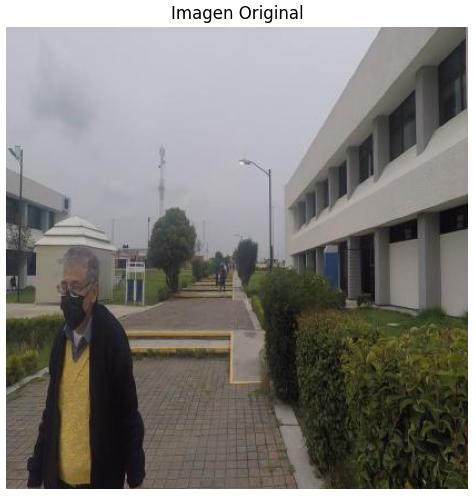
\includegraphics[width=0.6\textwidth]{images/sift_paso_1.png}
    \caption{Imagen original cargada.}
\end{figure}

\textbf{Paso 2: Conversión de la Imagen a Escala de Grises}

La imagen se convierte a escala de grises, ya que SIFT opera sobre la intensidad de los píxeles en lugar de los colores, lo que mejora la estabilidad de la detección de características.

\begin{figure}[H]
    \centering
    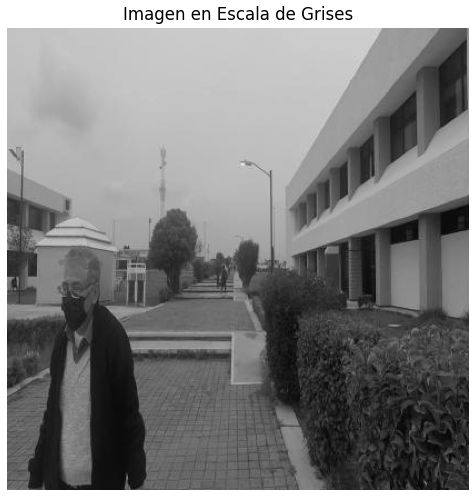
\includegraphics[width=0.6\textwidth]{images/sift_paso_2.png}
    \caption{Conversión a escala de grises.}
\end{figure}

\textbf{Paso 3: Configuración del Detector SIFT}
\par\vspace{0.5cm}

El detector \textbf{SIFT} requiere la configuración de varios parámetros clave que afectan la detección de características en la imagen:

\begin{itemize}
    \item \textbf{nfeatures = 5:} Número máximo de características a detectar. Si se establece en 0, se detectan todas las posibles características.
    \item \textbf{nOctaveLayers = 3:} Número de capas por octava en la pirámide Gaussiana.
    \item \textbf{contrastThreshold = 0.04:} Umbral para descartar características de bajo contraste.
    \item \textbf{edgeThreshold = 10:} Umbral para eliminar puntos en bordes poco definidos.
    \item \textbf{sigma = 1.6:} Desviación estándar inicial para el filtro Gaussiano.
\end{itemize}

Para la implementación, se ha utilizado la clase correspondiente en el módulo \texttt{algoritmos/sift.py}. 
\par\vspace{0.5cm}
En las pruebas iniciales, se estableció \texttt{nfeatures} en \textbf{5} para reducir la cantidad de puntos clave detectados, 
facilitando la visualización y comprensión teórica del proceso.
\par\vspace{0.5cm}

\textbf{Paso 4: Construcción de la Pirámide Gaussiana}
\par\vspace{0.5cm}

La pirámide Gaussiana se genera aplicando convoluciones sucesivas con filtros gausianos de distinta desviación estándar (\(\sigma\)), reduciendo la resolución de la imagen en cada octava. Este proceso permite analizar la imagen a diferentes escalas para detectar características invariantes.

\begin{figure}[H]
    \centering
    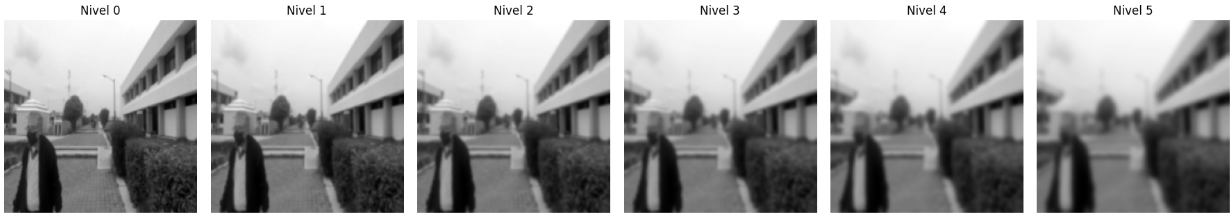
\includegraphics[width=1.1\textwidth]{images/sift_paso_3.1.png}
    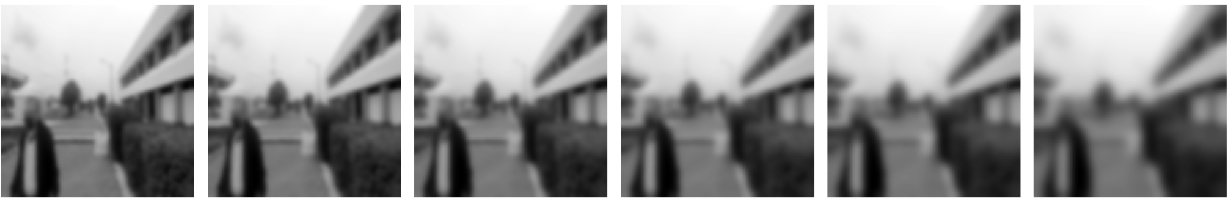
\includegraphics[width=0.9\textwidth]{images/sift_paso_3.2.png}
    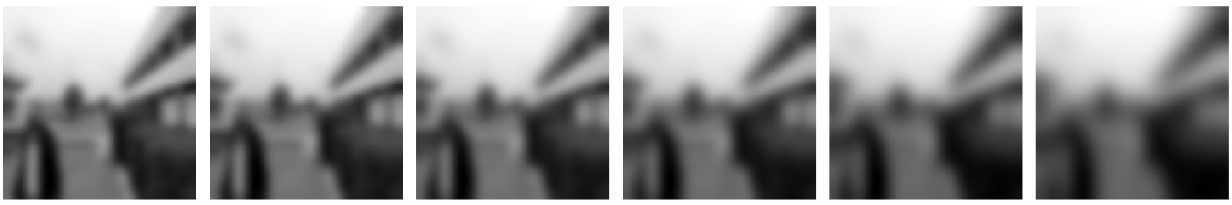
\includegraphics[width=0.7\textwidth]{images/sift_paso_3.3.png}
    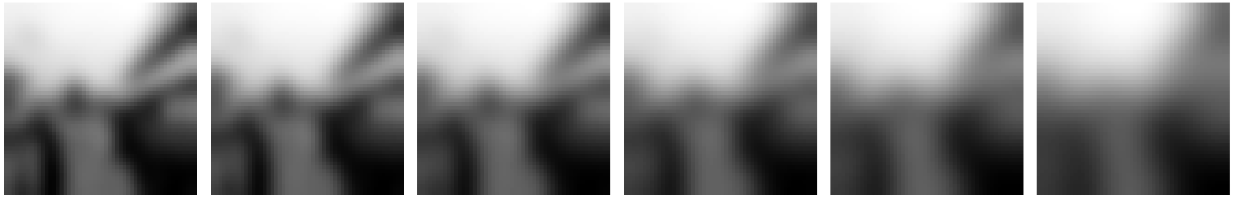
\includegraphics[width=0.4\textwidth]{images/sift_paso_3.4.png}
    \caption{Construcción de la Pirámide Gaussiana.}
\end{figure}

\textbf{Paso 5: Construcción de la Pirámide de Diferencia de Gaussianos (DoG)}

Después de generar la pirámide Gaussiana, se construye la pirámide de Diferencia de Gaussianos (DoG) restando imágenes consecutivas de la pirámide. Esto resalta las variaciones de intensidad entre niveles de suavizado, facilitando la detección de puntos de interés.

\begin{figure}[H]
    \centering
    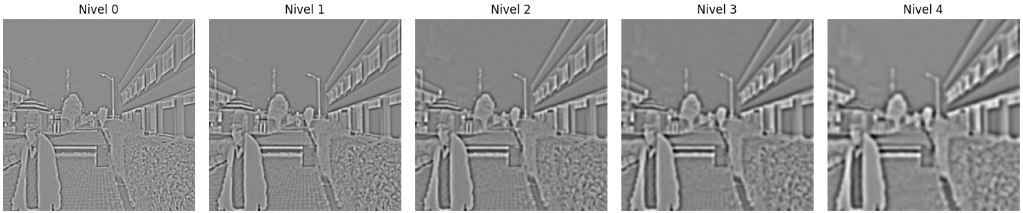
\includegraphics[width=1.1\textwidth]{images/sift_paso_4.1.png}
    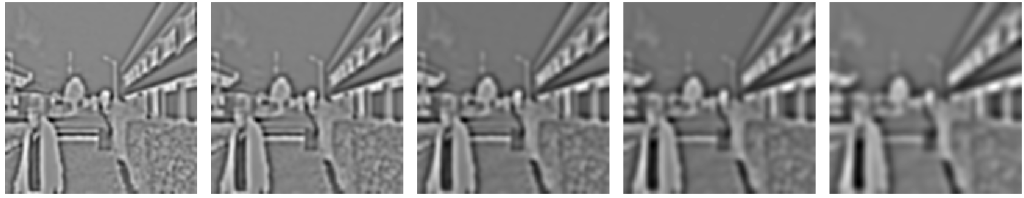
\includegraphics[width=0.9\textwidth]{images/sift_paso_4.2.png}
    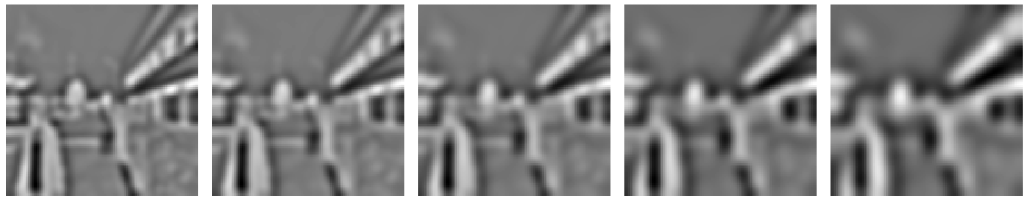
\includegraphics[width=0.7\textwidth]{images/sift_paso_4.3.png}
    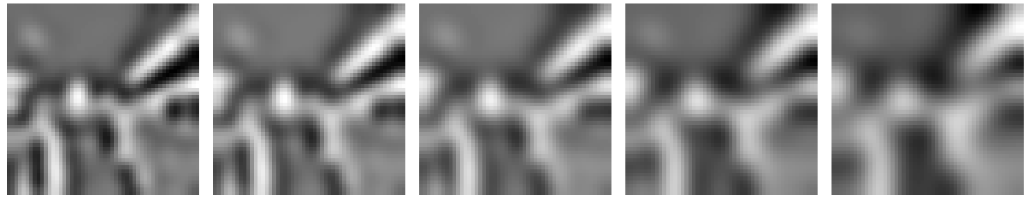
\includegraphics[width=0.4\textwidth]{images/sift_paso_4.4.png}
    \caption{Construcción de la Pirámide de Diferencia de Gaussianos (DoG).}
\end{figure}

\textbf{Paso 6: Detección de Keypoints}
\par\vspace{0.5cm}

Los keypoints se detectan identificando los extremos locales en la pirámide DoG. Se comparan píxeles con sus vecinos en los niveles superiores e inferiores de la pirámide para encontrar puntos máximos y mínimos. Como resultado, obtenemos 5 keypoints debido a la configuración propuesta anteriormente. 

\begin{figure}[H]
    \centering
    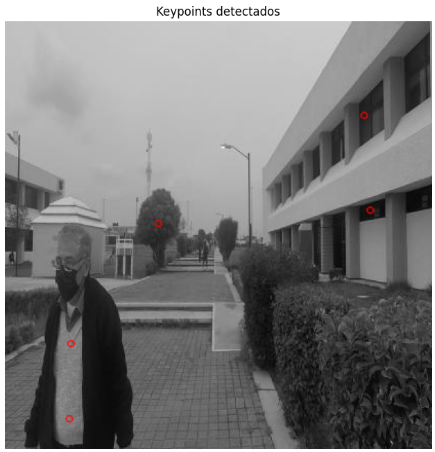
\includegraphics[width=0.6\textwidth]{images/sift_paso_5.1.png}
    \caption{Detección de 5 keypoints en la imagen.}
\end{figure}

En el caso de aplicar el valor 0 al parámetro \textbf{nfeatures}, se detectarían todas las características posibles en la imagen, lo que aumentaría significativamente el número de keypoints detectados, como se observa en la siguiente imagen:

\begin{figure}[H]
    \centering
    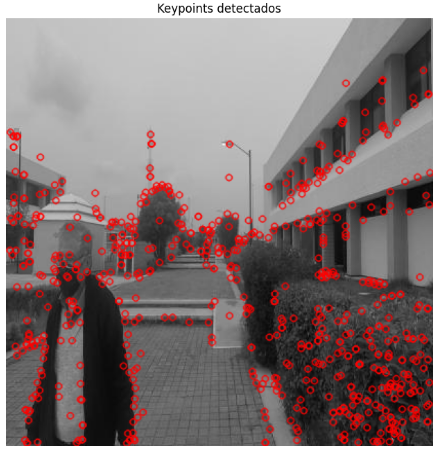
\includegraphics[width=0.6\textwidth]{images/sift_paso_5.png}
    \caption{Detección de todos los keypoints con \texttt{nfeatures} = 0.}
\end{figure}

\textbf{Paso 7: Asignación de Orientación a los Keypoints}
\par\vspace{0.5cm}

Cada keypoint recibe una orientación basada en los gradientes locales de la imagen. Esto permite que los descriptores sean invariables a la rotación.

\begin{figure}[H]
    \centering
    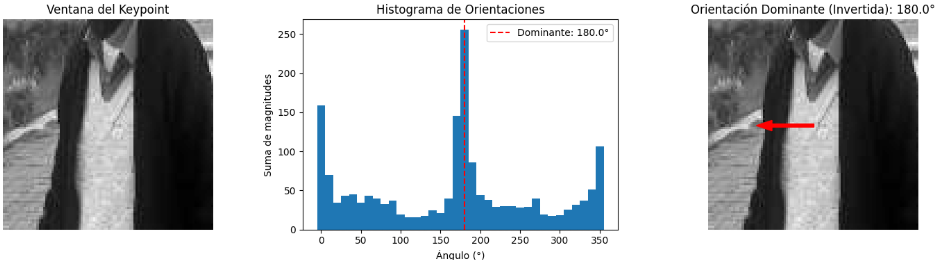
\includegraphics[width=1.1\textwidth]{images/sift_paso_6.1.png}
    \caption{Orientación asignada a cada keypoint.}
\end{figure}

\textbf{Paso 8: Visualización de los Keypoints con su Orientación}
\par\vspace{0.5cm}

Los keypoints detectados y sus orientaciones asignadas se visualizan para evaluar la robustez del algoritmo.

\begin{figure}[H]
    \centering
    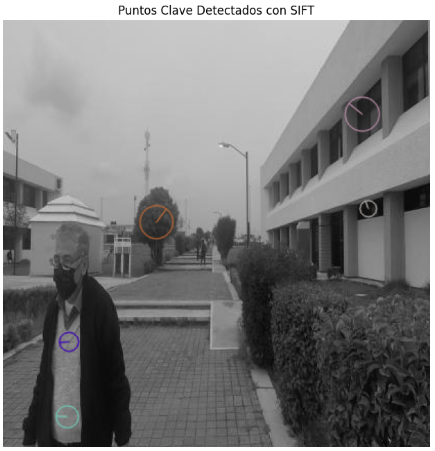
\includegraphics[width=0.6\textwidth]{images/sift_paso_7.1.png}
    \caption{Visualización de keypoints con orientación.}
\end{figure}

\textbf{Paso 9: Cálculo de Descriptores}
\par\vspace{0.5cm}

Cada keypoint se describe mediante un vector de características basado en la distribución de gradientes en su vecindad.

\begin{figure}[H]
    \centering
    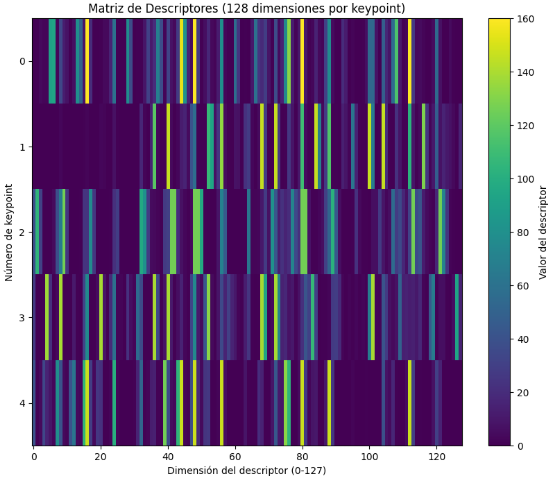
\includegraphics[width=0.8\textwidth]{images/sift_paso_8.png}
    \caption{Ejemplo de descriptor SIFT calculado.}
\end{figure}

Estos descriptores serán los que permitan al modelo de aprendizaje automático emparejar características entre diferentes imágenes, facilitando tareas como el reconocimiento de objetos y la detección de peatones en escenas complejas.


\subsubsection{HOG (Histogram of Oriented Gradients)}

El algoritmo HOG es una técnica eficaz para extraer y representar características locales en imágenes mediante el cálculo de gradientes orientados en pequeñas celdas. HOG se ha consolidado como una herramienta robusta para la detección de objetos, en particular para la identificación de peatones, ya que al combinar la descripción detallada de la estructura visual con la normalización de bloques, logra ser invariante frente a variaciones de iluminación, contraste y posición. 


\subsubsection{Proceso de Aplicación de HOG}

A continuación, se detallan los pasos seguidos en la implementación del algoritmo hog:
\par\vspace{0.5cm}

\textbf{Paso 1: Cargar y Mostrar la Imagen}
\par\vspace{0.5cm}

Antes de aplicar el algoritmo, se importan las librerías necesarias y se carga la imagen con la que se va a trabajar.

\begin{figure}[H]
    \centering
    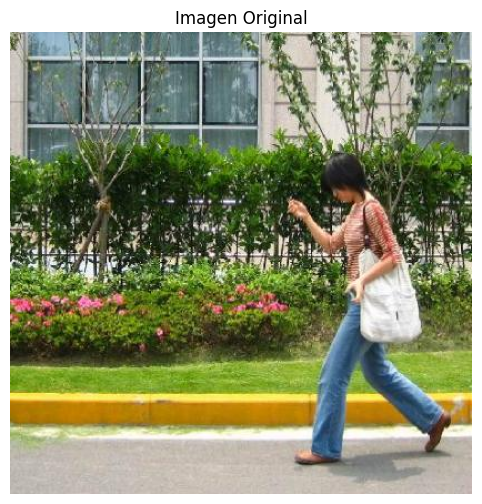
\includegraphics[width=0.5\textwidth]{images/hog_paso_1.png}
    \caption{Imagen original cargada.}
\end{figure}

\textbf{Paso2: Escalar la Imagen}
\par\vspace{0.5cm}

La imagen se escala para ajustar la resolución a un tamaño óptimo, lo que permite que el descriptor HOG capture de manera consistente los patrones y detalles esenciales, minimizando la carga computacional sin perder información relevante.

\begin{figure}[H]
    \centering
    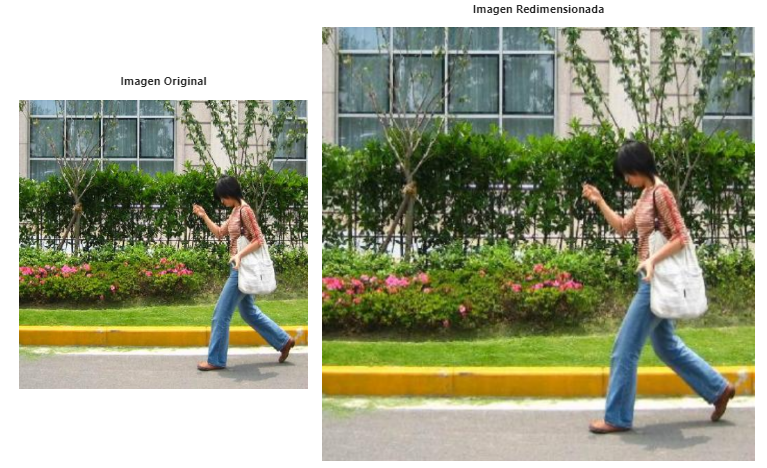
\includegraphics[width=0.6\textwidth]{images/hog_paso_2.png}
    \caption{Imagen original e imagen redimensionada.}
\end{figure}

\textbf{Paso 3: Configuración del detector HOG}
\par\vspace{0.5cm}

El detector HOG requiere la configuración de varios parámetros clave que afectan la detección de características en la imagen:
\begin{itemize}
    \item \textbf{cell\_size = (16,16):} Tamaño de cada celda en la que se divide la imagen.
    \item \textbf{block\_size = (2,2):} Número de celdas agrupadas para formar un bloque.
    \item \textbf{block\_stride = (8,8):} Desplazamiento en píxeles entre bloques.
    \item \textbf{nbins = 9:} Número de intervalos del histograma de orientaciones (cada bin abarca 20°).
    \item \textbf{win\_stride = (8,8):} Desplazamiento en píxeles de la ventana durante la detección.
    \item \textbf{padding = (8,8):} Acolchamiento aplicado a la imagen en el proceso de detección.
    \item \textbf{scale = 1.05:} Factor de escala para construir la pirámide de escalas.
    \item \textbf{bin\_width = 20:} Ancho (en grados) de cada bin en el histograma.
\end{itemize}

Para la implemnetación se ha utilizado la clase correspondiente en el módulo \texttt{algoritmos/hog.py}.
\par\vspace{0.5cm}

\textbf{Paso 4: Conversión de la Imagen a Escala de Grises}
\par\vspace{0.5cm}

La imagen se convierte a escala de grises para que HOG pueda centrarse exclusivamente en la estructura y forma de la imagen, lo que mejora la estabilidad de la extracción de gradientes y reducir la complejidad computacional.

\begin{figure}[H]
    \centering
    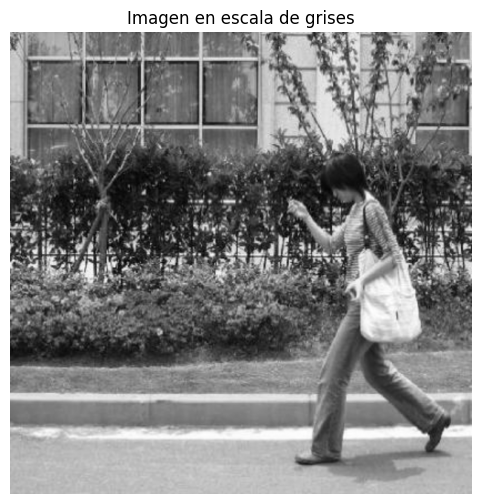
\includegraphics[width=0.4\textwidth]{images/hog_paso_4.png}
    \caption{Imagen en escala de grises.}
\end{figure}

\textbf{Paso 5: Cálculo de Gradientes}
\par\vspace{0.5cm}

El gradiente se calcula aplicando los operadores Sobel en las direcciones horizontal y vertical, obteniendo la magnitud y orientación de los cambios de intensidad en cada píxel. Esto permite resaltar los bordes y transiciones en la imagen, proporcionando información esencial sobre su estructura.

\begin{figure}[H]
    \centering
    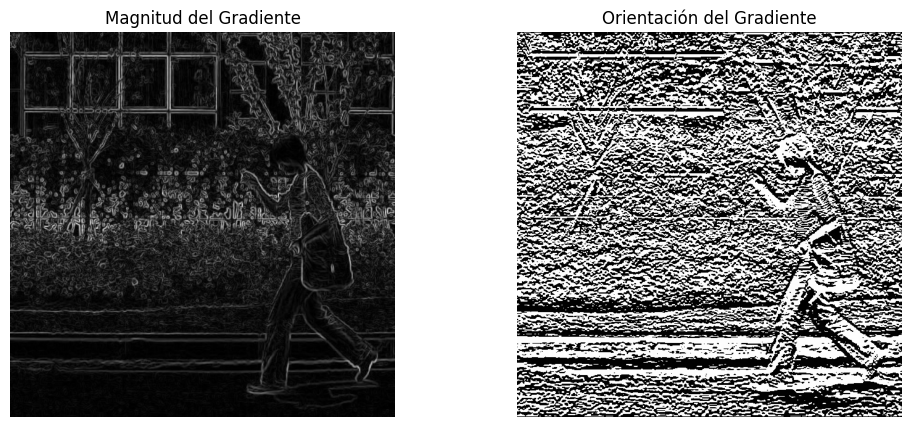
\includegraphics[width=0.8\textwidth]{images/hog_paso_5.png}
    \caption{Magnitud del gradiente y Orientación del gradiente.}
\end{figure}

\textbf{Paso 6: Cálculo del Histograma por celda}
\par\vspace{0.5cm}

En cada celda se construye un histograma que acumula las magnitudes de los gradientes según la orientación de cada píxel, lo que permite capturar y resumir la distribución local de bordes y transiciones en esa región de la imagen.

\begin{figure}[H]
    \centering
    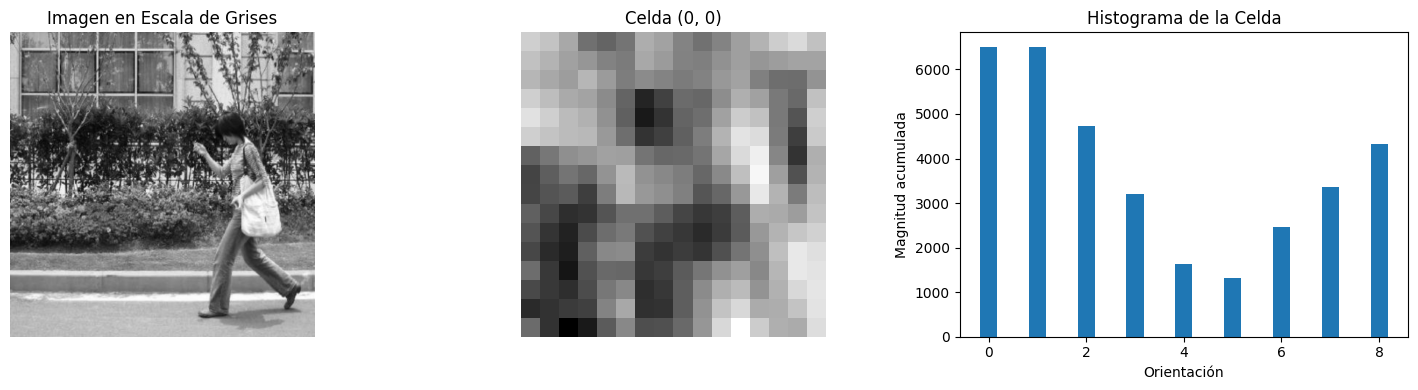
\includegraphics[width=0.9\textwidth]{images/hog_paso_6.png}
    \caption{Ejemplo de cálculo del histograma para la celda (0,0).}
\end{figure}

\textbf{Normalización de Bloques y Concatenación de Descriptores}
\par\vspace{0.5cm}

En este paso, los histogramas de las celdas se agrupan en bloques, y cada bloque se normaliza para reducir el efecto de variaciones en la iluminación y el contraste. Luego, los vectores normalizados de todos los bloques se concatenan para formar un descriptor global que resume la distribución de gradientes en toda la imagen.
\par\vspace{0.5cm}

\textbf{Paso 7: Visualización de los Descriptores HOG}
\par\vspace{0.5cm}

\begin{figure}[H]
    \centering
    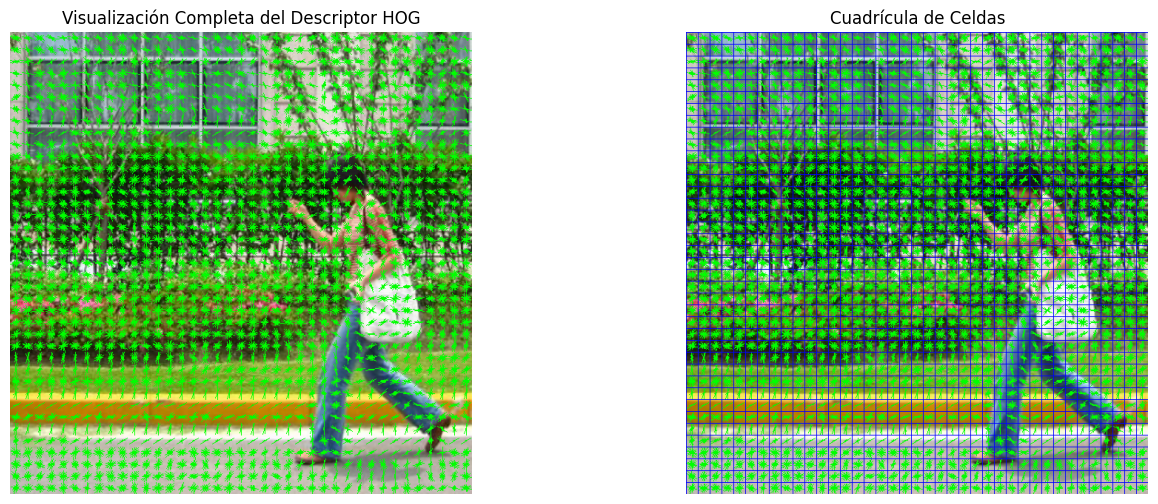
\includegraphics[width=1.0\textwidth]{images/hog_paso_7.png}
    \caption{Visualización del descriptor y Visualizalización del descriptor con celdas.}
\end{figure}

\subsection{Decisiones de Diseño}

\begin{itemize}
\item \textbf{Separación de los algoritmos en archivos independientes:} Cada método de detección (Harris, SURF, SIFT y HOG) se implementó en archivos de Python independientes dentro de una carpeta central denominada \texttt{algoritmos}.
\item \textbf{Presentación didáctica en Jupyter Notebooks:} Se desarrolló un \texttt{notebook.ipynb} por cada algoritmo donde se explican los algoritmos paso a paso.
\item \textbf{Experimentación con un banco de imágenes de prueba:} Se realizó una prueba con un conjunto de imágenes para entrenar un modelo \textbf{SVM} y predecir si en una imagen hay o no un peatón.
\item \textbf{Estructura organizada del proyecto:}  
    \begin{itemize}
        \item Se creó una carpeta \texttt{images} donde se almacenan los bancos de imágenes de entrenamiento del \textbf{SVM} y las pruebas para cada algoritmo. Las imágenes incluyen ejemplos con y sin personas, extraídas de \texttt{roboflow.com}.
        \item Se añadió una carpeta \texttt{doc} para documentar el desarrollo del proyecto y actualizarlo progresivamente.
        \item Se estableció una carpeta \texttt{machinelearning} dedicada específicamente al entrenamiento del modelo \textbf{SVM}.
        \item Los Jupyter Notebooks están ubicados en la raíz del proyecto para facilitar su acceso y ejecución.
    \end{itemize}
\end{itemize}

\newpage

\section{Experimentación}

La experimentación es una parte fundamental de este trabajo, ya que permite evaluar el rendimiento de los algoritmos implementados en combinación con el modelo \textbf{SVM} (Support Vector Machine). 
Para obtener resultados significativos, hemos realizado pruebas sistemáticas con las configuraciones más eficientes con cada algoritmo y un conjunto variado de imágenes.
\par \hspace{1cm}

Una vez implementados y probados los algoritmos de detección de características (\textbf{Harris, SURF, SIFT y HOG}), decidimos entrenar un modelo \textbf{SVM} utilizando un banco de datos con más de 1000 imágenes, en las que se incluyen ejemplos con y sin peatones. El objetivo es evaluar la capacidad del modelo para predecir correctamente la presencia de un peatón en una imagen.

\subsection{Preparación del Conjunto de Datos}

Para garantizar un entrenamiento adecuado del \textbf{SVM}, cada imagen del banco de datos fue sometida a un tratamiento previo, el cual depende del algoritmo de detección de características a evaluar. Este preprocesamiento incluyó:
\begin{itemize}
    \item Conversión a escala de grises (en los algoritmos que lo requieren).
    \item Aplicación del método de detección de características correspondiente (Harris, SURF, SIFT o HOG).
    \item Extracción de descriptores característicos de cada imagen.
    \item Normalización de los descriptores para mejorar la robustez del modelo.
\end{itemize}

\subsection{Entrenamiento del Modelo SVM}

Tras procesar el conjunto de datos, se procedió al entrenamiento del \textbf{SVM} con los descriptores extraídos de cada imagen. Para ello, se utilizó un conjunto de entrenamiento compuesto por imágenes etiquetadas en las que tomaba 
el valor true en caso de haber una o más personas (señalando su ubicación), y false en caso contrario, para diferenciar aquellas que contienen peatones de aquellas que no.


\subsection{Pruebas de Evaluación}

Una vez entrenado el modelo con los descriptores obtenidos de cada algoritmo, se realizó una prueba final con un conjunto de imágenes con y sin personas, que no habían sido utilizadas durante el entrenamiento. El objetivo era medir la eficiencia del modelo en la tarea de detección de peatones.

Cada imagen de prueba fue procesada de la misma manera que las imágenes de entrenamiento, aplicando el algoritmo de detección de características correspondiente y extrayendo sus descriptores. Posteriormente, estos descriptores fueron introducidos en el \textbf{SVM} entrenado para predecir si la imagen contenía un peatón o no.

\subsection{Resultados y Análisis}

Para evaluar el desempeño del modelo, se calcularon métricas como:
\begin{itemize}
    \item \textbf{Precisión}: Porcentaje de imágenes correctamente clasificadas.
    \item \textbf{Tiempo de Procesamiento}: Tiempo medio necesario para procesar una imagen.
\end{itemize}


\subsection{Resultados Obtenidos}


\newpage

\section{Manual de usuario}

El manual de usuario del proyecto se encuentra disponible en el archivo \texttt{README.md} dentro del repositorio del proyecto en GitHub. Dicho manual proporciona una guía detallada sobre el uso de la aplicación, incluyendo su instalación, configuración y funcionalidades principales.
\par\hspace{1cm}

Para acceder al manual de usuario, visite el siguiente enlace donde encontrará el repositorio del proyecto en GitHub:

\begin{center}
\url{https://github.com/Lidiajim/AnalisisDeAlgoritmosPID}
\end{center}
\newpage

\section{Conclusiones}

Se debe introducir una sección de conclusiones que incluyan propuestas claras de mejora o extensión del trabajo (por ejemplo, si no se han podido alcanzar todos los objetivos iniciales). También conclusiones sobre los resultados obtenidos, en qué medida difieren de los esperados. además, son apropiadas conclusiones sobre las desviaciones en cuanto a la planificación inicial, así como conclusiones sobre la experiencia de la realización del trabajo (lecciones aprendidas).
\newpage
\section{Autoevaluación}
A continuación se presenta la autoevaluación individual realizada por cada miembro del equipo según la rúbrica proporcionada:

\begin{table}[htbp]
  \centering
  \scriptsize
  \renewcommand{\arraystretch}{1.5}
  \setlength{\tabcolsep}{4pt}
  \begin{tabular}{|>{\raggedright\arraybackslash}p{2.8cm}|>{\raggedright\arraybackslash}p{3cm}|>{\raggedright\arraybackslash}p{3cm}|>{\raggedright\arraybackslash}p{3cm}|>{\raggedright\arraybackslash}p{3cm}|}
  \hline
  \multicolumn{5}{|c|}{\textbf{Rúbrica para evaluar los trabajos dirigidos}} \\
  \hline
  \textbf{Exposición} &  \textbf{Álvaro} & \textbf{Lidia} & \textbf{Víctor} & \textbf{Óscar} \\
  \hline
  Comprensión y dominio (puntuación triple)& Excelente & Excelente & Excelente & Excelente \\
  \hline
  Exposición didáctica & Excelente & Excelente & Excelente & Excelente\\
  \hline
  Integración del equipo & Excelente & Excelente & Excelente & Excelente \\
  \hline
  \textbf{Implementación} & \textbf{Álvaro} & \textbf{Lidia} & \textbf{Víctor} & \textbf{Óscar} \\
  \hline
  Objetivos (puntuación doble)& Excelente & Excelente & Excelente & Excelente \\
  \hline
  Aspectos didácticos & Excelente & Excelente & Excelente & Excelente \\
  \hline
  Experimentación y conclusiones & Excelente & Excelente & Excelente & Excelente \\
  \hline
  \textbf{Documentación} & \textbf{Álvaro} & \textbf{Lidia} & \textbf{Víctor} & \textbf{Óscar} \\
  \hline
  Contenidos & Excelente & Excelente & Excelente & Excelente \\
  \hline
  Divulgación contenidos & Excelente & Excelente & Excelente & Excelente \\
  \hline
  Bibliografía y recursos científicos & Excelente & Excelente & Excelente & Excelente \\
  \hline
  \end{tabular}
  \caption{Rúbrica para evaluar trabajos dirigidos (ponderada sobre 7 puntos)}
  \end{table}

  \newpage

\section{Tabla de tiempos}

El seguimiento del trabajo de cada participante del proyecto se ha dividido en cuatro fases claramente definidas, en las cuales cada miembro del equipo se centró en tareas específicas:
\begin{center}
  \begin{tabular}{|c|l|}
  \hline
  \textbf{Fase} & \textbf{Descripción y seguimiento asociado} \\
  \hline
  Fase 1 & Desarrollo de la idea inicial e investigación (seguimiento 0 y 1) \\
  Fase 2 & Implementación inicial mediante código (seguimiento 2) \\
  Fase 3 & Finalización de la implementación y documentación (seguimiento 3) \\
  Fase 4 & Preparación y presentación del proyecto (seguimiento 4) \\
  \hline
  \end{tabular}
  \end{center}

  \subsection*{Seguimiento Individual}

  \begin{center}
  \begin{tabular}{|c|c|c|c|c|}
  \hline
  Fase & Álvaro Ruiz Gutiérrez & Lidia Jiménez Soriano & Víctor Flores González & Óscar Menéndez Márquez \\
  \hline
  Fase 1 & 23,74 horas & 0 horas& 0 horas& 0 horas\\
  Fase 2 & 26,89 horas & 1 horas& 1 horas& 1 horas\\
  Fase 3 & x horas& 2 horas & 2 horas& 2 horas\\
  Fase 4 & x horas& 3 horas & 3 horas& 3 horas\\
  \hline
  \textbf{Total} & \textbf{70} & \textbf{70} & \textbf{70} & \textbf{70} \\
  \hline
  \end{tabular}
  \end{center}
  

Para consultar con mayor detalle las fechas específicas, tareas asignadas, tiempo dedicado por cada participante y otra información relevante, puedes acceder al siguiente enlace a la ficha de datos de Clockify: [LINK].
\newpage

\begin{thebibliography}{10}

  \bibitem{HARRIS}
  C. Harris y M. Stephens, \emph{A Combined Corner and Edge Detector}, Proceedings of The Fourth Alvey Vision Conference, pp. 147–151, 1988. Disponible en: \url{https://citeseerx.ist.psu.edu/document?repid=rep1&type=pdf&doi=88cdfbeb78058e0eb2613e79d1818c567f0920e2}
  
  \bibitem{SURF}
  H. Bay, T. Tuytelaars y L. Van Gool, \emph{Surf: Speeded up robust features}, en Computer Vision–ECCV 2006, Springer Berlin Heidelberg, pp. 404-417, 2006. Disponible en: \url{https://link.springer.com/chapter/10.1007/11744023_32}
  
  \bibitem{SIFT}
  I. Rey-Otero y M. Delbracio, \emph{Anatomy of the SIFT Method}, Image Processing On Line, vol. 4, pp. 370–396, 2014. Disponible en: \url{https://doi.org/10.5201/ipol.2014.82}
  
  \bibitem{HOG}
  N. Dalal y B. Triggs, \emph{Histograms of oriented gradients for human detection}, en IEEE Computer Society Conference on Computer Vision and Pattern Recognition (CVPR'05), San Diego, CA, EE.UU., vol. 1, pp. 886-893, 2005. DOI: 10.1109/CVPR.2005.177. Disponible en: \url{https://ieeexplore.ieee.org/abstract/document/1467360}
  
  \end{thebibliography}


\end{document}